\chapter{原子核的放射性}

\paragraph{原子核放射性发现史}
\begin{itemize}
	\item 1895年Röntgen发现X射线(\nobel{1901});
	\item 1896年Becquerel发现了铀的放射性质(\nobel{1903});
	\item 1898年Rutherford从Becquerel射线中分离出了$\alpha$和$\beta$粒子(\nobel{1908}\footnote{这居然是个化学奖。});
	\item 1900年Villard发现$\gamma$射线。
\end{itemize}

\begin{definition}{放射性术语}{radiation terminology}
	放射性:原子核自发地发射各种射线的现象。

	%放射性核素:能自发地发射各种射线的核素,也称为不稳定核素。

	衰变:原子核自发地发生转变的现象。
\end{definition}
原子核衰变的主要方式有$\alpha,\beta,\gamma$衰变、自发裂变、核子发射。

\paragraph{衰变纲图}\index{衰变纲图}一个典型的衰变纲图如下:
\begin{center}
		\includegraphics[page=3]{figures/tikz/layouts.pdf}
	\captionof{figure}{衰变纲图}
\end{center}
\begin{compactenum}
	\item 主核素$\nucli{137}{Cs}$,基态自旋$7/2$,宇称$+$,能量$0$,半衰期$\SI{30}{yr}$;
	\item 子核素$\nucli{137}{Ba}$,基态自旋$3/2$,宇称$+$;激发态自旋$11/2$,宇称$-$,能量$\SI{661.66}{keV}$,半衰期$\SI{2.5}{min}$;
	\item 反映的是$\beta^-$衰变,然后子核由激发态$\gamma$跃迁到基态的物理过程;
	\item 能量变化:$\SI{1175.63}{keV},\SI{513.97}{keV},\SI{661.66}{keV}$;
	\item 绝对强度(概率):基态-基态5.4\%,基态-激发态94.6\%,$\gamma$射线85.0\%,内转换电子9.6\%。
	% \item $\gamma$跃迁
\end{compactenum} 

\section{放射性衰变的基本规律}

放射性原子核是全同的,原子核的衰变是独立、随机的。因此不能预测某一原子核的衰变时刻,放射性衰变是一个统计过程。

单一放射性具有指数衰减规律
\begin{align}
	\dv{N(t)}t=-\lambda N(t)\implies N(t)=N(0)\e{-\lambda t}.
\end{align}
其中$\lambda$为衰变常数\index{衰变常数},表示一个原子核在单位时间内发生衰变的概率。

定义衰变率$J(t)$为$t$时刻单位时间内衰变的核数目\index{衰变率}
\[
	J(t):=-\dv{N(t)}t\equiv\lambda N(t)
\]
\begin{definition}{分支比}{ratio}
	当一个原子核有几种衰变方式时,$\lambda$等于分支$\lambda_i$之和。
	%$\lambda=\sum_i\lambda_i$
	定义分支比\index{分支比}
	\begin{align}
		R_i:=\frac{\lambda_i}\lambda,
	\end{align}
\end{definition}
在衰变纲图中,并不是全部的绝对强度均为分支比,绝对强度的和也不一定为1,但主核素衰变的强度就是分支比。
\begin{definition}{半衰期、平均寿命、衰变宽度}{}
	半衰期$T_{1/2}$:\index{半衰期}原子核衰变为50\%所需要的时间
	\begin{align}
		\e{-\lambda T_{1/2}}=\frac12\implies T_{1/2}:=\frac{\ln 2}\lambda\doteq\frac{0.693}\lambda.
	\end{align}
	平均寿命$\tau$\index{平均寿命}
	\begin{align}
		\tau:=\int\zti t\cdot\lambda\e{-\lambda t}\d t=\frac1\lambda.
	\end{align}
	衰变宽度$\varGamma$,\index{衰变宽度}由波函数的FWHM (过程略)得
	\begin{align}
		\varGamma:=\hbar/\tau=\hbar\lambda.
	\end{align}
\end{definition}
\begin{definition}{放射性活度}{activity}
	放射性活度(activity)定义为单位时间内发生衰变的原子核数\index{活度}\footnote{明明就和衰变率完全一样(流汗黄豆)}
	\begin{align}
		A(t):=-\dv{N(t)}t\equiv\lambda N(t),
	\end{align}
	其SI单位为Becquerel,$\SI{1}{Bq}=\SI{1}{\per s}$。
\end{definition}
历史上也采用过Curie作为单位(\SI{1}{g} $\nucli{226}{Ra}$的活度)二者的关系是
\begin{align}
	\SI{1}{Ci}=\SI{3.7e10}{Bq}.
\end{align}

% 活度大小与原子核数目$N(t)$以及衰变常数$\lambda$有关。废话

比活度\index{比活度}定义为单位质量放射源的放射性活度。

\section{递次衰变规律}

\paragraph{两次连续衰变规律}
考虑一个两次连续衰变
\[
	\nuc A\overset{\lambda_1}{\longrightarrow }\nuc B\overset{\lambda_2}{\longrightarrow }\nuc C~(\mathrm{stable})
\]
核素A是单一放射性衰变,服从简单的指数规律
\[
	N_1(t)=N_{10}\e{-\lambda_1t}
\]
B的变化包括两方面:
\[
	\dv{N_2(t)}t=\lambda_1N_1(t)-\lambda_2N_2(t),
\]
故
\[\label{N2}
	N_2(t)=N_{10}\frac{\lambda_1}{\lambda_2-\lambda_1}(\e{-\lambda_1t}-\e{-\lambda_2t}).\tag{$\ast$}
\]
C仅由B衰变得到:
\[
	\dv{N_3(t)}t=\lambda_2N_2(t),
\]
故
\[
	N_3(t)=N_{10}\frac{\lambda_1\lambda_2}{\lambda_2-\lambda_1}\fkh{\frac1{\lambda_1}(1-\e{-\lambda_1t})-\frac1{\lambda_2}(1-\e{-\lambda_2t})}.
\]
显然$N_1(t)+N_2(t)+N_3(t)=N_{10}$。
\paragraph{多次连续衰变规律}
对于$n$代连续放射性衰变过程:
\[
	\nuc A_1\overset{\lambda_1}{\longrightarrow }\nuc A_2\overset{\lambda_2}{\longrightarrow }\cdots\overset{\lambda_n}{\longrightarrow }\nuc A_{n+1}(\mathrm{stable})
\]
一般地,有
\[
	N_n(t)=N_{10}\sum_{i=1}^nc_i\e{-\lambda_it},\quad c_i=\dvd{\prod_{k=1}^{n-1}\lambda_k}{\prod_{k\neq i}(\lambda_k-\lambda_i)}.
\]
\paragraph{放射性平衡}考虑两次连续衰变,经过一定时间衰变可能会形成平衡。
\subparagraph{暂时平衡}$T_1>T_2$但$T_1$不很大,会形成暂时平衡。\index{暂时平衡}平衡特点:
\begin{compactenum}
	\item 子体与母核数目将建立起固定的比例关系;
	\item 子体按照母核的半衰期衰减。
\end{compactenum}
由式\eqref{N2},$N_2$和$A_2$存在极大值
\begin{align}
	\dv{N_2}t=0\implies t_\mathrm m=\frac{\ln\lambda_2-\ln\lambda_1}{\lambda_2-\lambda_1}.
\end{align}
$t_\mathrm m$时刻,$N_2$和$A_2$极大,且$A_1=A_2$。

$t>t_\mathrm m$时,$A_1<A_2$;$t\gg t_\mathrm m$时,子母核比例固定
%N_2(t)=\frac{\lambda_1}{\lambda_2-\lambda_1}N_1(t)(1-\e{-(\lambda_2-\lambda_1)t}).
\[
	\frac{N_2}{N_1}\doteq\frac{\lambda_1}{\lambda_2-\lambda_1},\quad\frac{A_2}{A_1}\doteq\frac{\lambda_2}{\lambda_2-\lambda_1}>1.
\]
\subparagraph{长期平衡}$T_1\gg T_2$且$T_1$很大。\index{长期平衡}虽然形式与暂时平衡相同,也有同样形式的$t_\mathrm m$,但$t\gg t_\mathrm m$后子母核活度相同:
\begin{align}
	\frac{A_2}{A_1}\doteq\frac{\lambda_2}{\lambda_2-\lambda_1}\doteq 1.
\end{align}
子核也是按着母核的半衰期衰变。

\subparagraph{不成平衡}$T_1<T_2$,时间足够长之后,母核就衰变完了,只有子核按自己的半衰期衰变。\index{不成平衡}

以上三种平衡均存在子母核活度关系的转折点$t_\mathrm m$,且受更短半衰期的核的影响更大。

\section{放射系}

地球上目前存在三个天然放射系:\index{放射系}
\begin{alignat*}{2}
	\text{钍系}\quad&^{232}_{~90}\mathrm{Th}&\quad T_{1/2}&=\SI{1.4e10}{yr},\\
	\text{铀系}\quad&^{238}_{~92}\mathrm{U}&\quad T_{1/2}&=\SI{4.468e9}{yr},\\
	\text{锕铀系}\quad&^{235}_{~92}\mathrm{U}&\quad T_{1/2}&=\SI{7.038e8}{yr}.
\end{alignat*}
这些都形成了长期平衡,子核的活度与母核相同。

放射系以$_{82}$Pb为终点,导致其母核$_{84}$Po半衰期一般都很短。

\section{放射规律的一些应用}

\paragraph{放射源活度修正}
\[
	A(t)=A(0)\e{-\lambda t}=\lambda N(0)\e{-\lambda t}.
\]
\paragraph{确定放射源性质}略,见讲义
\paragraph{确定放射源活度和制备时间}人工制备放射源时,如何确定源的活度和最佳制备时间?例
\[
	\nton+\nuc A\to\nuc B+\gamma,
\]
若粒子束的强度是一定的,则放射性核素B的产生率
\begin{align}
	P=N_{\mathrm{target}}\sigma_0\Phi,
\end{align}
是恒定不变的,式中$N_{\mathrm{target}}$是靶核A的数量,$\sigma_0$表示$\nton$与A的反应截面($\si{cm^2}$),$\Phi$表示中子注量率($\si{1/cm^2\cdot s}$)。

而生产的放射性核素又在不断地衰变,故
\[
	\dv{N(t)}t=P-\lambda N(t),
\]
故源的活度应为
\begin{align}
	A(t)=P(1-\e{-\lambda t}).
\end{align}
与$N_{\mathrm{target}},\sigma_0,\Phi,\lambda,t$五个因素有关。
定义饱和因子$S:=1-\e{-\lambda t}$。\index{饱和因子}
\paragraph{放射性鉴年法}$\nucli{14}C$具有$\beta^-$放射性
\[
	\nucli{14}C\to\nucli{14}N+\elc^-+\bar\nu_\elc,
\]
半衰期5700年。

而宇宙射线一直与大气层中的核发生反应,产生中子
\[
	\nton+\nucli{14}N\to\nucli{14}C+\pton.
\]
大气与生物体中$\nucli{12}C$与$\nucli{14}C$比例是一定的。生物死后体内$\nucli{14}C$不断衰变。
\paragraph{短寿命核素发生器}
核医学需要短寿命放射性核素作为标记核素,可以利用“母牛”生产这些核素并运输到医院等需要使用的地方。比如
\[
	\nucli{99}{Mo}\enspace\mathop{\semilongrightarrow}\limits^{\beta^-}_{\SI{66}{h}}\enspace\nucli{99m}{Tc}\enspace\mathop{\semilongrightarrow}\limits^{\mathrm{IT}}_{\SI{6}{h}}\enspace\nucli{99}{Tc},
\]
$t_\mathrm m=\SI{20.8}{h}$时,子核放射性活度最大,淋洗交换柱。

